\section{Algorytm \textit{ALERGIA}}  
\label{sec:alergia}  

Algorytm \textit{ALERGIA} \cite{ALERGIA} jest stosowany do indukcji stochastycznych gramatyk regularnych. W przeciwieństwie do \textit{RPNI} lub \textit{GIG}, które zakładają obecność zarówno przykładów pozytywnych, jak i negatywnych, \textit{ALERGIA} opiera się wyłącznie na zbiorze przykładów pozytywnych. Umożliwia to jego zastosowanie w sytuacjach, gdzie dostęp do przykładów negatywnych jest ograniczony lub niemożliwy.  

Algorytm ten konstruuje deterministyczny stochastyczny automat skończony (DSFA) na podstawie drzewa akceptacji prefiksów (PTA) utworzonego z dostępnych danych. Proces uogólniania polega na łączeniu stanów automatu, przy jednoczesnym zachowaniu zgodności ze statystycznym rozkładem prawdopodobieństwa przejść między stanami. Decyzje o scalaniu są podejmowane na podstawie testów statystycznych, które zapewniają, że wynikowy model zachowuje probabilistyczne własności danych wejściowych.  

Jedną z kluczowych cech algorytmu \textit{ALERGIA} jest jego zdolność do indukcji gramatyk stochastycznych, co czyni go szczególnie przydatnym w zastosowaniach wymagających modelowania niepewności lub probabilistycznych wzorców zachowań. Dzięki swojej efektywności obliczeniowej algorytm ten znajduje zastosowanie w zadaniach takich jak rozpoznawanie wzorców, analiza sekwencji biologicznych oraz modelowanie języka naturalnego.

Algorytm działa iteracyjnie, testując kompatybilność stanów i łącząc te, które są statystycznie zgodne. Proces kończy się, gdy żadne dalsze scalenie nie jest możliwe bez naruszenia kryteriów statystycznych. Dzięki temu wynikowy automat nie tylko reprezentuje język generowany przez dane treningowe, ale także umożliwia estymację prawdopodobieństwa generacji nowych ciągów.


\subsection{Metoda}  
Algorytm \textit{ALERGIA} pozwala na indukcję deterministycznego stochastycznego automatu skończonego (DSFA), który przybliża rozkład prawdopodobieństwa danych wejściowych. Proces ten obejmuje następujące kroki:  

\begin{enumerate}  
    \item \textbf{Budowa akceptora drzewa prefiksów (PTA):}  
        Zbiór przykładów pozytywnych jest używany do zbudowania deterministycznego automatu reprezentującego dokładnie wszystkie sekwencje w danych.  
    \item \textbf{Iteracyjne łączenie stanów:}  
        Algorytm analizuje pary stanów w PTA i testuje ich zgodność statystyczną. Łączenie stanów jest realizowane tylko wtedy, gdy nie narusza statystycznej zgodności z danymi.  
    \item \textbf{Sprawdzanie zgodności:}  
        Kompatybilność stanów jest oceniana za pomocą testu Hoeffding'a.  
    \item \textbf{Zakończenie:}  
        Algorytm kończy działanie, gdy żadne dalsze scalenie stanów nie jest możliwe bez naruszenia zgodności statystycznej. Ostateczny automat aproksymuje rozkład probabilistyczny danych wejściowych.  
\end{enumerate}


\subsection{Formalizacja}  
W tej sekcji przedstawiono matematyczne podstawy algorytmu \textit{ALERGIA} oraz definicje kluczowych pojęć, które umożliwiają precyzyjne opisanie jego działania. Algorytm ten wykorzystuje akceptor drzewa prefiksów (PTA) jako strukturę początkową z definicji \ref{def:pta}. Proces formalizacji skupia się na mechanizmach scalania stanów, które pozwalają na stopniowe upraszczanie automatu przy jednoczesnym zachowaniu zgodności z probabilistycznymi wzorcami danych wejściowych.  

\begin{definition}[DSFA]  
\label{def:dsfa}
Stochastyczny, skończony automat deterministyczny to piątka uporządkowana
\[ 
A = (Q, \Sigma, \delta, q_0, P), 
\]
gdzie:  
\begin{itemize}  
    \item \( Q \) – skończony zbiór stanów,  
    \item \( \Sigma \) – alfabet,  
    \item \( \delta : Q \times \Sigma \to Q \) – funkcja przejścia,  
    \item \( q_0 \in Q \) – stan początkowy,  
    \item \( P: Q \times \Sigma \to [0, 1] \) – funkcja prawdopodobieństwa przejść, spełniająca:  
    \[
    \sum_{a \in \Sigma} P(q, a) \leq 1, \quad \forall q \in Q, \quad a \in \Sigma.
    \]  
\end{itemize}
\end{definition}

Automat \( A \) generuje język stochastyczny, w którym każda sekwencja symboli z \( \Sigma \) jest akceptowana z określonym prawdopodobieństwem, wyznaczanym przez funkcję \( P \).

\begin{definition}[Test Hoeffding’a]  
\label{def:hoeffding_test}
Test Hoeffding’a w algorytmie ALERGIA jest wykorzystywany do porównania dwóch stanów \( q_1, q_2 \) poprzez wyznaczenie granicy tolerancji \( \epsilon \), która określa maksymalną dopuszczalną różnicę między ich rozkładami. Granica tolerancji \( \epsilon \) jest obliczana jako:  
\[
\epsilon = \sqrt{\frac{1}{2} \ln\left(\frac{2}{\alpha}\right)} \left( \frac{1}{\sqrt{n_1}} + \frac{1}{\sqrt{n_2}} \right),
\]
gdzie:  
\begin{itemize}  
    \item \( n_1, n_2 \) – liczba obserwacji w stanach \( q_1 \) i \( q_2 \),  
    \item \( \alpha \) – poziom ufności określający dopuszczalny margines błędu.  
\end{itemize}  
\end{definition}

Test Hoeffding’a to statystyczna metoda oceny zgodności dwóch rozkładów prawdopodobieństwa, bazująca na nierówności Hoeffding’a. W kontekście algorytmu \textit{ALERGIA} test ten służy do sprawdzania, czy różnice między obserwowanymi częstościami przejść w stanach automatu można uznać za przypadkowe, czy też są one statystycznie istotne. W algorytmie \textit{ALERGIA} test Hoeffding’a porównuje rozkłady przejść pomiędzy stanami automatu. Jeśli różnice są mniejsze niż wyznaczony próg tolerancji, stany są uznawane za zgodne statystycznie i mogą zostać scalone. 

\begin{definition}[Zgodność stanów]  
\label{def:alergia_state_compatibility}
Dwa stany \( q_1, q_2 \in Q \) są uznawane za zgodne (kompatybilne), jeżeli spełnione są dwa warunki:  
\begin{enumerate}
    \item Funkcja prawdopodobieństwa przejść \( P \) dla każdego symbolu \( a \in \Sigma \) spełnia:  
    \[
    |P(q_1, a) - P(q_2, a)| \leq \epsilon.
    \]  
    \item Prawdopodobieństwa terminacji \( P_F \) spełnia:
    \[
    |P_F(q_1) - P_F(q_2)| \leq \epsilon,
    \]  
    gdzie \( \epsilon \) jest granicą wyznaczoną przez test Hoeffding’a.
\end{enumerate}
\end{definition} 

\begin{definition}[Łączenie stanów w \textit{ALERGIA}]  
\label{def:alergia_state_merging}  
Łączenie dwóch stanów \( q_1, q_2 \in Q \) w stochastycznym, skończonym automacie deterministycznym (DSFA) \( A = (Q, \Sigma, \delta, q_0, P) \) polega na zintegrowaniu informacji o przejściach oraz rozkładach prawdopodobieństwa w jeden wspólny stan. Proces ten obejmuje następujące kroki:  

\begin{enumerate}  
    \item Wierzchołek reprezentujący stan \( q_2 \) zostaje przypisany jako poddrzewo do stanu \( q_1 \) poprzez modyfikację drzewa prefiksów.  
    \item Funkcja przejścia zostaje zaktualizowana:  
    \[
    \delta'(q, a) =
    \begin{cases}  
        \delta(q_1, a) & \text{jeśli } \delta(q, a) = q_2, \\  
        \delta(q, a) & \text{w przeciwnym przypadku.}  
    \end{cases}  
    \]  
    \item Przejścia oraz rozkłady prawdopodobieństwa dla symboli \( a \) są łączone poprzez uśrednienie wagowe:  
    \[
    P'(q, a) = \frac{n_1 \cdot P(q_1, a) + n_2 \cdot P(q_2, a)}{n_1 + n_2},
    \]  
    gdzie \( n_1 \) i \( n_2 \) oznaczają liczby obserwacji dla stanów \( q_1 \) i \( q_2 \).  
    \item Następnie wszystkie dzieci stanu \( q_2 \) zostają przeniesione do stanu \( q_1 \). Jeśli stan \( q_1 \) posiada już przejście dla danego symbolu, częstotliwości są sumowane. W przeciwnym przypadku tworzony jest nowy węzeł:  
    \[
    P'(q_1, a) = P(q_1, a) + P(q_2, a).
    \]  
    Proces ten jest kontynuowany rekurencyjnie dla wszystkich dzieci stanu \( q_2 \).  
\end{enumerate}  
\end{definition}  

Łączenie stanów jest przeprowadzane wyłącznie wtedy, gdy dwa stany oraz pary ich dzieci odpowiadające przejściom tych samych symboli spełniają kryteria zgodności określone w definicji \ref{def:alergia_state_compatibility}. Scalanie obejmuje także sumowanie obserwacji oraz prawdopodobieństw dla poddrzew, co zapewnia zachowanie struktury probabilistycznej danych wejściowych. Proces kończy się, gdy żadne dalsze połączenia nie spełniają warunków zgodności.  

% \subsection{Złożoność}  
% Algorytm \textit{ALERGIA} cechuje się złożonością wielomianową, zależną od rozmiaru danych wejściowych. W analizie złożoności czasowej i pamięciowej uwzględniamy następujące parametry:  
% \begin{itemize}  
%     \item \(|S^+|\) - liczba przykładów pozytywnych,  
%     \item \( l^+ \) - maksymalna długość ciągu w \( S^+ \),  
%     \item \(|Q|\) - liczba stanów w automacie,  
%     \item \(|\Sigma|\) - liczba symboli w alfabecie.  
% \end{itemize}  

% \paragraph*{Złożoność czasowa.}  
% Algorytm \textit{ALERGIA} składa się z dwóch głównych etapów: budowy drzewa prefiksowego oraz iteracyjnego scalania stanów.  

% \subparagraph*{Budowa drzewa prefiksowego (PTA).}  
% Pierwszy etap polega na utworzeniu drzewa prefiksowego (Prefix Tree Acceptor, PTA) na podstawie zbioru przykładów pozytywnych. Każde słowo jest dodawane do drzewa, a jego prefiksy są reprezentowane jako kolejne węzły. Proces ten wymaga analizy wszystkich przykładów oraz ich symboli, co prowadzi do złożoności:  
% \[
% O(|S^+| \cdot l^+).
% \]  

% \subparagraph*{Iteracyjne scalanie stanów.}  
% Drugi etap obejmuje iteracyjne porównywanie par stanów pod kątem zgodności, wykorzystując test Hoeffding’a. Każda para stanów jest sprawdzana pod względem zgodności prawdopodobieństw przejść i terminacji, a następnie wykonywane są rekurencyjne analizy następników. Sprawdzenie każdej pary stanów obejmuje:
% \begin{itemize}  
%     \item Porównanie prawdopodobieństw przejść dla wszystkich symboli w alfabecie \( \Sigma \).  
%     \item Rekurencyjne sprawdzenie zgodności następników.  
%     \item Ewentualne scalanie stanów, co wiąże się z aktualizacją przejść i prawdopodobieństw.  
% \end{itemize}  

% Złożoność iteracyjnego scalania stanów wynosi:  
% \[
% O(|Q|^4 \cdot |\Sigma|).
% \]  

% \subparagraph*{Złożoność rzeczywista.}  
% W praktyce rzeczywista złożoność algorytmu jest często znacznie niższa niż teoretyczna granica. Wynika to z dwóch głównych czynników:  
% \begin{enumerate}
%     \item Algorytm wcześnie scala zgodne stany, zmniejszając liczbę analizowanych stanów w kolejnych iteracjach.  
%     \item Stany znajdujące się na końcu porządku przetwarzania (liście drzewa) mają niewielu następców lub w ogóle ich nie posiadają, co ogranicza liczbę rekurencyjnych wywołań.  
% \end{enumerate}  

% Z tego powodu empiryczna złożoność algorytmu jest często bliższa:  
% \[
% O(|Q|^3 \cdot |\Sigma|).
% \]  

% \paragraph*{Łączna złożoność.}  
% Podsumowując, całkowita złożoność czasowa algorytmu obejmuje budowę drzewa oraz iteracyjne porównania i scalania stanów:  
% \[
% O(|S^+| \cdot l^+ + |Q|^4 \cdot |\Sigma|).
% \]

% \paragraph*{Zależność liczby stanów \( Q \).}  
% Liczba stanów \( |Q| \) w automacie jest bezpośrednio zależna od danych wejściowych. W najgorszym przypadku każde słowo o długości \( l^+ \) wnosi dokładnie \( l^+ \) nowych stanów. Przy \( |S^+| \) przykładach liczba stanów może wynosić:  
% \[
% |Q| \leq |S^+| \cdot l^+.
% \]  
% Z tego powodu rzeczywista złożoność algorytmu jest silnie powiązana z rozmiarem zbioru przykładów i długością słów.   
% \[
% O((|S^+| \cdot l^+)^4 \cdot |\Sigma|).
% \]


% \paragraph*{Złożoność pamięciowa}  
% Algorytm przechowuje następujące struktury:  
% \begin{itemize}  
%     \item \textbf{Drzewo prefiksowe (PTA):}  
%     PTA składa się z \( O(|S^+| \cdot l^+) \) stanów, z których każdy może mieć do \( |\Sigma| \) przejść. Wymagana przestrzeń pamięci wynosi:  
%     \[
%     O(|S^+| \cdot l^+ \cdot |\Sigma|).
%     \]  

%     \item \textbf{Statystyki przejść:}  
%     Dla każdego stanu przechowywane są rozkłady prawdopodobieństw oraz dane statystyczne, co daje dodatkowy koszt pamięciowy:  
%     \[
%     O(|S^+| \cdot l^+).
%     \]  
% \end{itemize}  

% Łączna złożoność pamięciowa wynosi:  
% \[
% O(|S^+| \cdot l^+ \cdot |\Sigma|).
% \]  

% \paragraph*{Czynniki wpływające na złożoność}  
% Efektywność algorytmu \textit{ALERGIA} zależy przede wszystkim od liczby przykładów pozytywnych (\( S^+ \)) oraz długości słów (\( l^+ \)), które determinują rozmiar drzewa prefiksowego i liczbę stanów do analizy. Dodatkowo, większy alfabet (\( |\Sigma| \)) zwiększa liczbę możliwych przejść, co wpływa zarówno na czas obliczeń, jak i wymagania pamięciowe.

\subsection{Przykład działania}  
Aby zilustrować działanie algorytmu \textit{ALERGIA}, rozważmy prosty przykład danych wejściowych opisujących sekwencje wyników rzutów monetą. Każdy wynik jest oznaczony symbolem \( H \) (orzeł) lub \( T \) (reszka).

\paragraph*{Dane wejściowe.}  
Zbiór przykładów pozytywnych (\( S^+ \)):  
\[
S^+ = \{H, H, T, HH, HT, TH, TT, HHH\}.
\]  

\paragraph*{Krok 1: Konstrukcja drzewa prefiksowego (PTA).}  
Na podstawie danych pozytywnych algorytm buduje drzewo prefiksowe (Prefix Tree Acceptor, PTA), które reprezentuje dokładnie wszystkie obserwowane sekwencje. Każdy stan odpowiada prefiksowi słów z \( S^+ \), a przejścia są etykietowane symbolami \( H \) lub \( T \). Wynik tego kroku można zobaczyć na rysunku \ref{fig:alergia_example_0}. 

\begin{figure}[ht]
    \centering
    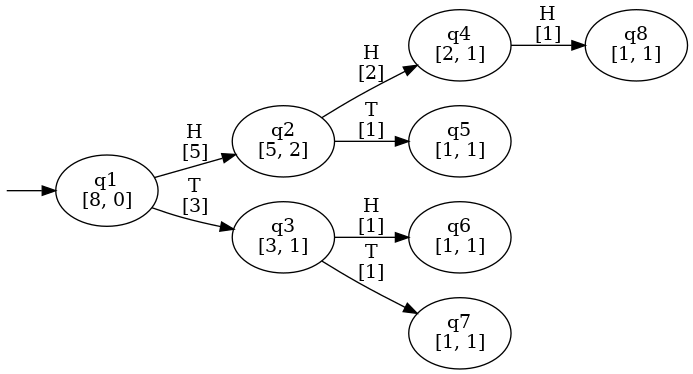
\includegraphics[width=0.8\textwidth]{images/run_example/alergia/0.png}
    \caption{Drzewo prefiksowe (PTA) skonstruowane dla \( S^+ \).}
    \label{fig:alergia_example_0}
\end{figure}

\paragraph*{Krok 2: Próba scalania stanów \( q_1 \) i \( q_2 \).}  
Algorytm rozpoczyna proces od analizy zgodności pierwszej pary stanów \( q_1 \) i \( q_2 \). Weryfikacja odbywa się na podstawie rozkładów prawdopodobieństw przejść oraz prawdopodobieństwa terminacji w obu stanach.  

\paragraph*{Dane stanów:}  
\begin{itemize}  
    \item \( q_1 \): \( n = 8, F = 0 \), przejścia: \( H[5], T[3] \).  
    \item \( q_2 \): \( n = 5, F = 2 \), przejścia: \( H[2], T[1] \).  
\end{itemize}  

\paragraph*{Sprawdzenie terminacji:}  
Prawdopodobieństwo terminacji dla każdego stanu:  
\[
P_F(q_1) = \frac{0}{8} = 0, \quad P_F(q_2) = \frac{2}{5} = \num{0.4},
\]

Różnica:  
\[
|P_F(q_1) - P_F(q_2)| = |0 - \num{0.4}| = \num{0.4}.
\]

\paragraph*{Tolerancja Hoeffding’a:}  
Przy poziomie ufności \( \alpha = \num{1.7} \) oraz liczbach obserwacji \( n_1 = 8 \) i \( n_2 = 5 \), granica zgodności \( \epsilon \) jest obliczana na podstawie wzoru:  
\[
\epsilon = \sqrt{\frac{\ln(2 / \alpha)}{2}} \left( \frac{1}{\sqrt{n_1}} + \frac{1}{\sqrt{n_2}} \right)
\]
\[
\epsilon \approx \num{0.228}.
\]

\paragraph*{Porównanie:}  
Ponieważ \( \num{0.4} > \num{0.228} \), stany \( q_1 \) i \( q_2 \) \textbf{nie mogą zostać połączone}.

\paragraph*{}

\paragraph*{Krok 3: Scalanie stanów \( q_2 \) i \( q_3 \).}  
Po odrzuceniu scalania stanów \( q_1 \) i \( q_2 \), algorytm przechodzi do analizy zgodności pary stanów \( q_2 \) i \( q_3 \).

\paragraph*{Dane stanów:}  
\begin{itemize}  
    \item \( q_2 \): \( n = 5, F = 2 \), przejścia: \( H[2], T[1] \), 
    \item \( q_3 \): \( n = 3, F = 1 \), przejścia: \( H[1], T[1] \).  
\end{itemize}  

\paragraph*{Test Hoeffding’a:}  
Prawdopodobieństwo terminacji dla każdego stanu:  
\[
P(q_2, H) = \frac{2}{5} = \num{0.4}, \quad P(q_3, H) = \frac{1}{3} \approx \num{0.333},
\]
\[
P(q_2, T) = \frac{1}{5} = \num{0.2}, \quad P(q_3, T) = \frac{1}{3} \approx \num{0.333},
\]
\[
P_F(q_2) = \frac{2}{5} = \num{0.4}, \quad P_F(q_3) = \frac{1}{3} \approx \num{0.333}.
\]

Różnica:  
\[
|P(q_2, H) - P(q_3, H)| \approx |\num{0.4} - \num{0.333}| = \num{0.067},
\]
\[
|P(q_2, T) - P(q_3, T)| \approx |\num{0.2} - \num{0.333}| = \num{0.133},
\]
\[
|P_F(q_2) - P_F(q_3)| \approx |\num{0.4} - \num{0.333}| = \num{0.067}.
\]

\paragraph*{Tolerancja Hoeffding’a:}  
Przy poziomie ufności \( \alpha = \num{1.7} \) oraz liczbach obserwacji \( n_1 = 5 \) i \( n_2 = 3 \), granica zgodności \( \epsilon \) jest obliczana na podstawie wzoru:  
\[
\epsilon = \sqrt{\frac{\ln(2 / \alpha)}{2}} \left( \frac{1}{\sqrt{n_1}} + \frac{1}{\sqrt{n_2}} \right)
\]
\[
\epsilon \approx \num{0.318}.
\]

\paragraph*{Porównanie:}  
Ponieważ:  
\[
|P(q_2, H) - P(q_3, H)| < \num{0.318}, \quad
\]
\[
|P(q_2, T) - P(q_3, T)| < \num{0.318}, \quad
\]
\[
|P_F(q_2) - P_F(q_3)| < \num{0.318},
\]  
stany \( q_2 \) i \( q_3 \) \textbf{są zgodne}. Aby mogły zostać połączone musimy sprawdzić rekurencyjnie zgodność dzieci stanu $q_3$ z odpowiednikami z gałęzi $q_2$, tj. $q_4$ i $q_6$ oraz $q_5$ i $q_7$. Analogiczne obliczenia wykazują zgodność wszystkich tych par stanów. Wynik tego kroku przedstawiono na rysunku \ref{fig:alergia_example_1}.  

\begin{figure}[ht]
    \centering
    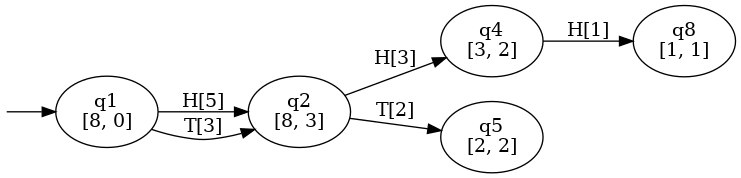
\includegraphics[width=0.8\textwidth]{images/run_example/alergia/1.png}
    \caption{Graf po scaleniu stanów \( q_2 \) i \( q_3 \).}
    \label{fig:alergia_example_1}
\end{figure}

\paragraph*{Krok 4: Scalanie stanów \( q_4 \) i \( q_8 \).}  
Po wcześniejszym scaleniu stanów \( q_2 \) i \( q_3 \), \( q_4 \) i \( q_6 \) oraz \( q_5 \) i \( q_7 \), algorytm przechodzi do następnej zgodnej pary stanów \( q_4 \) i \( q_8 \). Stan \( q_4 \) po wcześniejszym scaleniu z \( q_6 \) posiada \( n = 3, F = 2 \) oraz przejście \( H[1] \). Stan \( q_8 \) ma \( n = 1, F = 1 \) i brak przejść. Obliczenia są przeprowadzane analogicznie do wcześniejszych kroków. Porównanie prawdopodobieństw przejść oraz terminacji pokazuje, że różnice mieszczą się w zakresie tolerancji Hoeffding’a. Dzięki temu stany mogą zostać połączone, tworząc nowy stan \( q_4 \) o wartościach \( n = 4, F = 3 \) oraz przejściem zwrotnym \( H[1] \). Wynik tego kroku przedstawiono na rysunku \ref{fig:alergia_example_2}.  

\begin{figure}[ht]
    \centering
    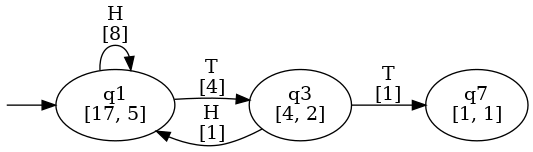
\includegraphics[width=0.8\textwidth]{images/run_example/alergia/2.png}
    \caption{Graf po scaleniu stanów \( q_4 \) i \( q_8 \).}
    \label{fig:alergia_example_2}
\end{figure}  

\paragraph*{Krok 5: Scalanie stanów \( q_4 \) i \( q_5 \).}  
Po wcześniejszych krokach, w których scalono stany \( q_2 \) z \( q_3 \), \( q_4 \) z \( q_6 \) oraz \( q_5 \) z \( q_7 \), algorytm przechodzi do analizy zgodności pary stanów \( q_4 \) i \( q_5 \). Stan \( q_4 \) po wcześniejszych operacjach posiada \( n = 3, F = 2 \) z przejściem zwrotnym \( H[1] \), natomiast stan \( q_5 \) ma \( n = 2, F = 2 \) i brak przejść. Obliczenia Hoeffding’a przeprowadzone w sposób analogiczny do wcześniejszych kroków pokazują, że różnice w rozkładach prawdopodobieństw przejść oraz terminacji mieszczą się w zakresie tolerancji. Dzięki temu stany zostają połączone, tworząc nowy stan \( q_4 \) z wartościami \( n = 5, F = 4 \) oraz przejściem zwrotnym \( H[1] \). Wynikowy graf można zobaczyć na rysunku \ref{fig:alergia_example_3}.

\begin{figure}[ht]
    \centering
    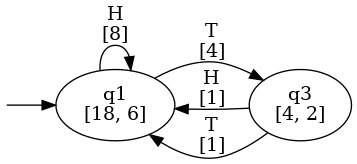
\includegraphics[width=0.8\textwidth]{images/run_example/alergia/3.png}
    \caption{Graf po scaleniu stanów \( q_4 \) i \( q_5 \).}
    \label{fig:alergia_example_3}
\end{figure}  

\paragraph*{Przekształcenie do postaci probabilistycznej.}  
W ostatnim kroku przekształcamy graf do postaci probabilistycznej. Prawdopodobieństwa terminacji oraz przejść są obliczane w sposób analogiczny do poprzednich kroków, uwzględniając wartości dla każdego stanu oraz przejść między nimi. Finalna postać grafu probabilistycznego reprezentuje rozkład danych wejściowych i umożliwia estymację nowych sekwencji. Wynikowy automat stochastyczny odwzorowuje prawdopodobieństwa przejść oraz terminacji, zapewniając zgodność probabilistyczną z danymi treningowymi. Wyniki tych kroków przedstawiono na rysunkach \ref{fig:alergia_example_4}.  

\begin{figure}[ht]
    \centering
    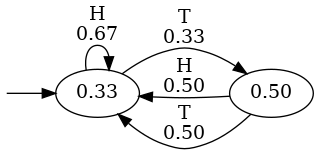
\includegraphics[width=0.8\textwidth]{images/run_example/alergia/4.png}
    \caption{Graf z probabilistycznymi przejściami i terminacjami.}
    \label{fig:alergia_example_4}
\end{figure}  

\paragraph*{Podsumowanie:}  
Algorytm zakończył proces scalania, redukując liczbę stanów i upraszczając strukturę automatu. Wynikowy automat stochastyczny zachowuje zgodność probabilistyczną z danymi wejściowymi, reprezentując ich rozkłady prawdopodobieństwa w sposób bardziej uogólniony. Finalna postać automatu pozwala na estymację nowych sekwencji zgodnych z rozkładem danych treningowych.  
